\begin{frame}{Photoemission from Flat Metal}
  \begin{columns}
  \begin{column}{0.54\linewidth}
  \begin{center}
  \begin{tikzpicture}
    \filldraw
      [fill=black!50]
      (0,0) 
      node [name=photocathode1,below right]{}
      node [below=1mm of photocathode1] {}
      -- ++(1,0)
      -- ++(0,-5)
      node [name=source,midway] {} 
      -- ++(-1,0)
      -- cycle
    ;
    \draw
      [-latex,ultra thick,green] 
      ($(source) + (45:3.5)$) 
      -- (source.east)
      node [name=laser label,pos=0.3,black,fill=white] {Laser ($\lambda$)}
    ;
    \fill
      [blue!30]
      (source.east)
      -- ++(3,6mm)
      -- ++(0,-12mm)
      -- cycle
    ;
    \draw
      [-latex,ultra thick,blue]
      (source.east)
      -- ++(3,6mm)
    ;
    \draw
      [-latex,ultra thick,blue]
      (source.east)
      -- ++(3,-6mm)
      node [name=electron label,at end,black,below,align=center]{Photoemitted\\Electrons}
    ;
    \draw
      [dashed]
      (source)
      -- ++(4,0)
    ;
%     \draw 
%       ($(source) + (1,0)$) 
%       arc (0:41:1)
%       node [right=0.3] {$\theta$}
%     ;
  \end{tikzpicture}
  \end{center}
  \end{column}
  \begin{column}{0.44\linewidth}
%     \begin{equation*}
%       P(\theta) = \smashoperator{\int\limits_{0}^{\Delta E = \hbar \omega - \Phi}} T(E,\theta) \dx{E}
%     \end{equation*}
%     \centerline{\tiny Assuming flat fermi function}
    \begin{figure}
      \centering
      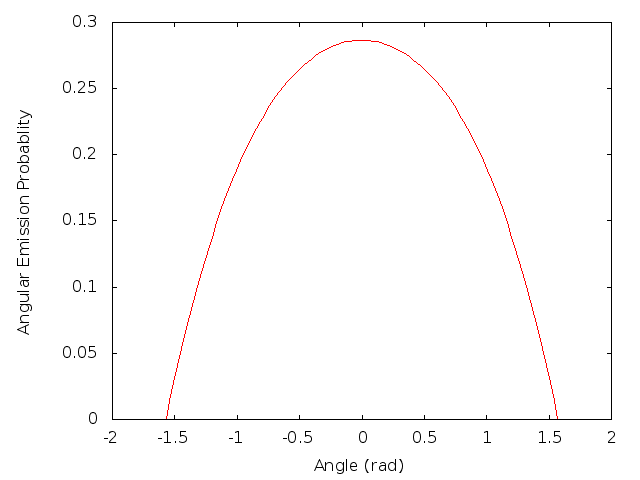
\includegraphics[width=0.9\linewidth]{Angle}
    \end{figure}
  \end{column}
  \end{columns}
\end{frame}


